% !TEX root = master.tex


\chapter{The BGK Model}
\label{Ch:BGK}
%\pagenumbering{arabic}




This chapter covers the kinetic gas model, the BGK model, on which a model order reduction will be performed in the following. In addition the SOD-shocktube, on which the BGK model will be tested is discussed.\\
The BGK model is valid for a broad range of rarefaction levels. Ranging from continuum flows, where the Navier-Stokes equations can be utilized to highly rarefied regimes. Rarefaction levels are labeled with the so called Knudsen number \(\Kn\) first introduced by danish physicist Martin Knudsen \cite{Bernard}. the Knudsen number is given by
\begin{equation}
	\Kn = \frac{\lambda}{l}, 
\end{equation}
where \(\lambda\) is the mean free path of a particle and \(l\), some domain specific length as the diameter of a tube for example. \Cref{Fig:ExpKN} shows a possible partitioning of \(\Kn\) into specific regimes, which is quiet comfortable. Though no clear cut can be applied to different values of \(\Kn\). The boundaries are particularly blurry \cite{schaaf}.
\begin{figure}[H]
	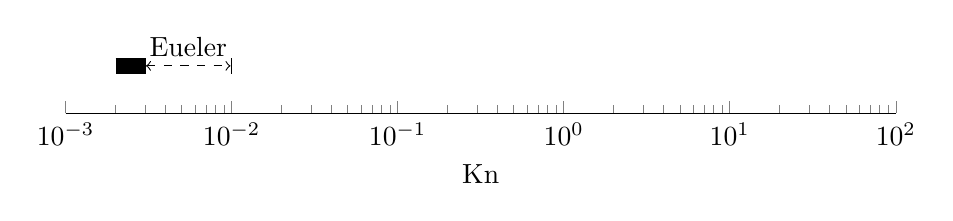
\begin{tikzpicture}
\begin{axis}[
    y=3cm,            % y unit vector
    hide y axis,        % hide the y axis
    xmode = log,        % logarithmic x axis
    axis x line*=bottom,% only show the bottom x axis line, without an arrow tip
    xmin=1e-3, xmax=1e2,% range for the x axis
    xlabel = Kn,
    width=\textwidth,
]
\addplot [no markers, line width=6pt] table {%
0.002 1
0.003 1
};
\draw [|<->|,dashed] (axis cs:0.003,1) -- (axis cs: 0.01,1) node[midway,above] {Eueler};
\end{axis}
%\begin{scope}[decoration=brace]
%	\draw [decorate] (current axis.south-|0.003) -- (current axis.south-|0.01) node[midway,above] {Eueler};
%\end{scope}
%\draw [] (axis cs:0.25,2.1) node[above] {\(T\)};
%\begin{scope}[decoration=brace]
%\pgfdecorationsegmentamplitude=5pt
%\draw[decorate] (T2.south east) -- (T0.south west) node[midway,below=\pgfdecorationsegmentamplitude] {Part 1};
%\draw[decorate] (T14.south east) -- (T3.south west) node[midway,below=\pgfdecorationsegmentamplitude] {Part 2};
%\draw[decorate] (T20.south east) -- (T15.south west) node[midway,below=\pgfdecorationsegmentamplitude] {Part 3};
%\end{scope}
\end{tikzpicture}
	\caption{Partitioning of \(\Kn\), the Knudsen number, into levels of rarefaction. The Euler equations can be used up to approximately \(\Kn < 0.01\) and describe a \glqq continuum flow\grqq{}. A \grqq slip flow\grqq{} can be defined in the interval \(0.01 < \Kn < 0.1\), termed as slightly rarefied in \cite{schaaf}. Here the Navier-stokes-Fourrier equations yield accurate results. From \(\Kn > 0.1\) onwards (transition regime, kinetic regime and free flight) the rarefaction increases steadily and only kinetic gas models deliver reasonable computations. The BGK model can be used for all rarefaction levels.}
	\label{Fig:ExpKN}
\end{figure}
\section{Space and Velocity Discretization, Moments and Conservation}
The BGK model was introduced by, and named after, physicists Prabhu L. Bhatnagar, Eugene P. Gross and Max Krook in 1954 \cite{BGK}. It is an approximation of the standard Boltzmann transport equation. More precisely the right hand side of the Boltzmann equation is approximated by the BGK operator 
\begin{equation}
\partial_t f + v \partial_x f = \frac{1}{\tau} (M_f - f) \text{,}
\label{Eq:BGK}
\end{equation}
which can be found in \cite{puppo2019kinetic}.It features the relaxation time \(\tau(x,t)\), the Maxwellian distribution \(M_f\) and \(f(t,v,x)\) the probability of a gas particle having a microscopic velocity \(v\) in phase space \((t,v,x)\). The right hand side is a source term describing the distance between the current probability density function \(f\) and it's equilibrium solution \(M_f\). Evidently when \(f = M_f\) the right hand side becomes zero. More precisely equilibirum is reached. A time scale for which \(f\) transitions into equilibrium is given by \(\tau\) which can be defined with
\begin{equation}
	\tau^{-1} = \frac{\rho(x,t)T^{1-\nu}(x,t)}{\Kn}\mathrm{,}
\end{equation}
taken from \cite{Bernard}. Through \(\tau\) the viscosity exponent \(\nu\), density \(\rho\), temperature \(T\) and Knudsen number \(\Kn\) additionally establish a scaling factor for the right hand side of the BGK model. The Maxwellian distribution \(M_f\) is defined by \(\rho(x,t)\), \(T(x,t)\) and \(u(x,t)\) the macroscopic velocity
\begin{equation}
M_f = \frac{\rho(x,t)}{(2\pi R T(x,t))^{\frac{3}{2}}}\exp(-\frac{(v - u(x,t))^2}{2 R T(x,t)}) \text{.}
\end{equation} 
The left hand side of the BGK model is the Boltzmann transport equation for \(f(t,v,x)\) with microscopic transport velocity \(v\).
In one dimension, the BGK model needs to be evaluated for the three independent variables \(x\), \(v\) and \(t\) as seen above. Furthermore in three dimensions one needs to include the evaluation at \((x,y,z)\) in space and \((v_x,v_y,v_z)\) in velocity space. Note that in this thesis the BGK model is discussed in one dimension only.\\ 
Now what makes the BGK model especially attractive for model order reduction?
The fruitfullness of performing a model order reduction on the BGK model becomes clearer when looking at it's space and velocity discretization
\begin{equation}
	\partial_t f_{j,k} = -(v_k)_1D_x f|_{j,k}(t) + \frac{1}{\tau}({M_f}_{j,k}(t) - f_{j,k}(t)) \text{,}
	\label{Eq:Discrete BGK}
\end{equation}
found in \cite{puppo2019kinetic}. Here a uniform grid is considered with \(x_j = j\Delta x\), \(j \in \mathbb{Z}\), \(v_k = k\Delta v\), \(k \in \mathbb{Z}\) and \(t^n = n \Delta t\), \(n \in \mathbb{N}\) on which \(f_{j,k} = f(t,v_k,x_j)\) and \({M_f}_{j,k} = M_f(x_j,v_k,t)\) are evaluated at point \((x_j,v_k)\) in a time instance \(t\). For brevity \(D_x f|_{j,k}\) is the discrete space derivative at \((x_j,v_k)\). Now the partial differential equation (PDE) in \cref{Eq:BGK} is broken down into a system of ordinary differential equations (ODE's) in time, for which every ODE is a linear advection equation with constant scalar speed \(v_k\) and a source term.\\
To continue let's consider \(K\) to be the number of gridpoints in velocity and \(J\) to be the number of grid points in space. Then a total of \(KJ\) first order differential equations need to be evaluated in 1D. Obviously in three dimensions the system of ODE's inflates up to \(K^3J^3\) first order differential equations. This in turn drives the evaluation of the BGK model at the edge of intractability for dense meshes in 3D and all together motivate for a reduced order model.\\
A closer look on the discretization in velocity space yields the necessity to compute the moments of \(f\) and provides a system of conservative equations.\\  
\begin{wrapfigure}{r}{0.5\textwidth}
	\vspace{-10pt}
	\scalebox{.9}{% This file was created by tikzplotlib v0.9.6.
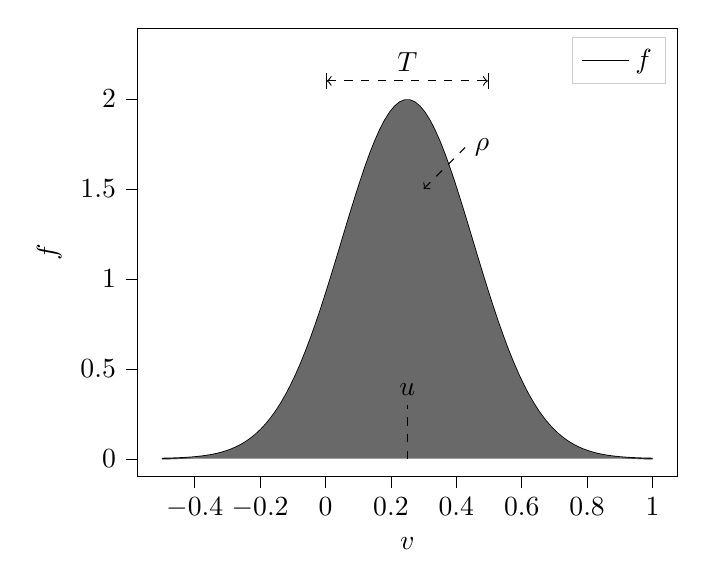
\begin{tikzpicture}

\begin{axis}[
legend cell align={left},
legend style={fill opacity=0.8, draw opacity=1, text opacity=1, draw=white!80!black},
tick align=outside,
tick pos=left,
x grid style={white!69.0196078431373!black},
xlabel={\(v\)},
xmin=-0.575, xmax=1.075,
xtick style={color=black},
y grid style={white!69.0196078431373!black},
ylabel={\(f\)},
ymin=-0.0978129180007683, ymax=2.39285680307655,
ytick style={color=black}
]

\addplot [semithick, black]
table {%
	-0.5 0.00176297841183723
	-0.484848484848485 0.00233549990938288
	-0.46969696969697 0.00307623995021814
	-0.454545454545455 0.0040287289903483
	-0.439393939393939 0.00524594088238899
	-0.424242424242424 0.00679182087082491
	-0.409090909090909 0.00874292085377632
	-0.393939393939394 0.0111901101946249
	-0.378787878787879 0.0142403174963827
	-0.363636363636364 0.018018244420721
	-0.348484848484849 0.0226679772544878
	-0.333333333333333 0.0283544060972295
	-0.318181818181818 0.0352643460570684
	-0.303030303030303 0.0436072406856785
	-0.287878787878788 0.0536153162176469
	-0.272727272727273 0.0655430473059348
	-0.257575757575758 0.0796657922473926
	-0.242424242424242 0.0962774595613305
	-0.227272727272727 0.115687079522804
	-0.212121212121212 0.138214174964358
	-0.196969696969697 0.164182856129127
	-0.181818181818182 0.193914604924168
	-0.166666666666667 0.227719764364528
	-0.151515151515151 0.265887808434693
	-0.136363636363636 0.308676534413689
	-0.121212121212121 0.356300391543538
	-0.106060606060606 0.408918233661475
	-0.0909090909090909 0.466620855301653
	-0.0757575757575757 0.529418736525693
	-0.0606060606060606 0.597230476778283
	-0.0454545454545454 0.669872437749538
	-0.0303030303030303 0.747050135179608
	-0.0151515151515151 0.828351915965591
	0 0.91324542694511
	0.0151515151515151 1.00107732368077
	0.0303030303030303 1.09107658129022
	0.0454545454545454 1.18236165636822
	0.0606060606060607 1.2739516126026
	0.0757575757575758 1.36478116780159
	0.0909090909090909 1.45371945330681
	0.106060606060606 1.53959210603912
	0.121212121212121 1.62120614747867
	0.136363636363636 1.69737695187443
	0.151515151515151 1.76695647690227
	0.166666666666667 1.82886183207001
	0.181818181818182 1.88210320029322
	0.196969696969697 1.92581011126961
	0.212121212121212 1.95925509432898
	0.227272727272727 1.98187381354832
	0.242424242424242 1.99328090666395
	0.257575757575758 1.99328090666395
	0.272727272727273 1.98187381354832
	0.287878787878788 1.95925509432898
	0.303030303030303 1.92581011126961
	0.318181818181818 1.88210320029322
	0.333333333333333 1.82886183207001
	0.348484848484849 1.76695647690227
	0.363636363636364 1.69737695187443
	0.378787878787879 1.62120614747867
	0.393939393939394 1.53959210603912
	0.409090909090909 1.45371945330681
	0.424242424242424 1.36478116780159
	0.439393939393939 1.2739516126026
	0.454545454545455 1.18236165636822
	0.46969696969697 1.09107658129022
	0.484848484848485 1.00107732368077
	0.5 0.91324542694511
	0.515151515151515 0.828351915965591
	0.53030303030303 0.747050135179608
	0.545454545454545 0.669872437749538
	0.560606060606061 0.597230476778283
	0.575757575757576 0.529418736525694
	0.590909090909091 0.466620855301653
	0.606060606060606 0.408918233661474
	0.621212121212121 0.356300391543538
	0.636363636363636 0.308676534413689
	0.651515151515152 0.265887808434693
	0.666666666666667 0.227719764364528
	0.681818181818182 0.193914604924168
	0.696969696969697 0.164182856129127
	0.712121212121212 0.138214174964358
	0.727272727272727 0.115687079522804
	0.742424242424242 0.0962774595613305
	0.757575757575758 0.0796657922473926
	0.772727272727273 0.0655430473059348
	0.787878787878788 0.0536153162176469
	0.803030303030303 0.0436072406856785
	0.818181818181818 0.0352643460570684
	0.833333333333333 0.0283544060972294
	0.848484848484849 0.0226679772544878
	0.863636363636364 0.018018244420721
	0.878787878787879 0.0142403174963826
	0.893939393939394 0.0111901101946249
	0.909090909090909 0.00874292085377631
	0.924242424242424 0.00679182087082491
	0.939393939393939 0.00524594088238899
	0.954545454545455 0.0040287289903483
	0.96969696969697 0.00307623995021814
	0.984848484848485 0.00233549990938288
	1 0.00176297841183723
};
\addlegendentry{\(f\)}

\path [draw=none, fill=white!41.1764705882353!black]
(axis cs:-0.5,0.00176297841183723)
--(axis cs:-0.484848484848485,0.00233549990938288)
--(axis cs:-0.46969696969697,0.00307623995021814)
--(axis cs:-0.454545454545455,0.0040287289903483)
--(axis cs:-0.439393939393939,0.00524594088238899)
--(axis cs:-0.424242424242424,0.00679182087082491)
--(axis cs:-0.409090909090909,0.00874292085377632)
--(axis cs:-0.393939393939394,0.0111901101946249)
--(axis cs:-0.378787878787879,0.0142403174963827)
--(axis cs:-0.363636363636364,0.018018244420721)
--(axis cs:-0.348484848484849,0.0226679772544878)
--(axis cs:-0.333333333333333,0.0283544060972295)
--(axis cs:-0.318181818181818,0.0352643460570684)
--(axis cs:-0.303030303030303,0.0436072406856785)
--(axis cs:-0.287878787878788,0.0536153162176469)
--(axis cs:-0.272727272727273,0.0655430473059348)
--(axis cs:-0.257575757575758,0.0796657922473926)
--(axis cs:-0.242424242424242,0.0962774595613305)
--(axis cs:-0.227272727272727,0.115687079522804)
--(axis cs:-0.212121212121212,0.138214174964358)
--(axis cs:-0.196969696969697,0.164182856129127)
--(axis cs:-0.181818181818182,0.193914604924168)
--(axis cs:-0.166666666666667,0.227719764364528)
--(axis cs:-0.151515151515151,0.265887808434693)
--(axis cs:-0.136363636363636,0.308676534413689)
--(axis cs:-0.121212121212121,0.356300391543538)
--(axis cs:-0.106060606060606,0.408918233661475)
--(axis cs:-0.0909090909090909,0.466620855301653)
--(axis cs:-0.0757575757575757,0.529418736525693)
--(axis cs:-0.0606060606060606,0.597230476778283)
--(axis cs:-0.0454545454545454,0.669872437749538)
--(axis cs:-0.0303030303030303,0.747050135179608)
--(axis cs:-0.0151515151515151,0.828351915965591)
--(axis cs:0,0.91324542694511)
--(axis cs:0.0151515151515151,1.00107732368077)
--(axis cs:0.0303030303030303,1.09107658129022)
--(axis cs:0.0454545454545454,1.18236165636822)
--(axis cs:0.0606060606060607,1.2739516126026)
--(axis cs:0.0757575757575758,1.36478116780159)
--(axis cs:0.0909090909090909,1.45371945330681)
--(axis cs:0.106060606060606,1.53959210603912)
--(axis cs:0.121212121212121,1.62120614747867)
--(axis cs:0.136363636363636,1.69737695187443)
--(axis cs:0.151515151515151,1.76695647690227)
--(axis cs:0.166666666666667,1.82886183207001)
--(axis cs:0.181818181818182,1.88210320029322)
--(axis cs:0.196969696969697,1.92581011126961)
--(axis cs:0.212121212121212,1.95925509432898)
--(axis cs:0.227272727272727,1.98187381354832)
--(axis cs:0.242424242424242,1.99328090666395)
--(axis cs:0.257575757575758,1.99328090666395)
--(axis cs:0.272727272727273,1.98187381354832)
--(axis cs:0.287878787878788,1.95925509432898)
--(axis cs:0.303030303030303,1.92581011126961)
--(axis cs:0.318181818181818,1.88210320029322)
--(axis cs:0.333333333333333,1.82886183207001)
--(axis cs:0.348484848484849,1.76695647690227)
--(axis cs:0.363636363636364,1.69737695187443)
--(axis cs:0.378787878787879,1.62120614747867)
--(axis cs:0.393939393939394,1.53959210603912)
--(axis cs:0.409090909090909,1.45371945330681)
--(axis cs:0.424242424242424,1.36478116780159)
--(axis cs:0.439393939393939,1.2739516126026)
--(axis cs:0.454545454545455,1.18236165636822)
--(axis cs:0.46969696969697,1.09107658129022)
--(axis cs:0.484848484848485,1.00107732368077)
--(axis cs:0.5,0.91324542694511)
--(axis cs:0.515151515151515,0.828351915965591)
--(axis cs:0.53030303030303,0.747050135179608)
--(axis cs:0.545454545454545,0.669872437749538)
--(axis cs:0.560606060606061,0.597230476778283)
--(axis cs:0.575757575757576,0.529418736525694)
--(axis cs:0.590909090909091,0.466620855301653)
--(axis cs:0.606060606060606,0.408918233661474)
--(axis cs:0.621212121212121,0.356300391543538)
--(axis cs:0.636363636363636,0.308676534413689)
--(axis cs:0.651515151515152,0.265887808434693)
--(axis cs:0.666666666666667,0.227719764364528)
--(axis cs:0.681818181818182,0.193914604924168)
--(axis cs:0.696969696969697,0.164182856129127)
--(axis cs:0.712121212121212,0.138214174964358)
--(axis cs:0.727272727272727,0.115687079522804)
--(axis cs:0.742424242424242,0.0962774595613305)
--(axis cs:0.757575757575758,0.0796657922473926)
--(axis cs:0.772727272727273,0.0655430473059348)
--(axis cs:0.787878787878788,0.0536153162176469)
--(axis cs:0.803030303030303,0.0436072406856785)
--(axis cs:0.818181818181818,0.0352643460570684)
--(axis cs:0.833333333333333,0.0283544060972294)
--(axis cs:0.848484848484849,0.0226679772544878)
--(axis cs:0.863636363636364,0.018018244420721)
--(axis cs:0.878787878787879,0.0142403174963826)
--(axis cs:0.893939393939394,0.0111901101946249)
--(axis cs:0.909090909090909,0.00874292085377631)
--(axis cs:0.924242424242424,0.00679182087082491)
--(axis cs:0.939393939393939,0.00524594088238899)
--(axis cs:0.954545454545455,0.0040287289903483)
--(axis cs:0.96969696969697,0.00307623995021814)
--(axis cs:0.984848484848485,0.00233549990938288)
--(axis cs:1,0.00176297841183723)
--cycle;
\addlegendimage{area legend, draw=none, fill=white!41.1764705882353!black}




\draw [dashed,|<->|] (axis cs:0,2.1) -- (axis cs:0.5,2.1);
\draw [] (axis cs:0.25,2.1) node[above] {\(T\)};
\draw [dashed] (axis cs:0.25,0)--(axis cs:0.25,0.3);
\draw [] (axis cs:0.25,0.3) node[above] {\(u\)};
\draw [dashed,<-] (axis cs:0.3,1.5)-- +(15pt,15pt) node[right] {\(\rho\)};
\end{axis}
\end{tikzpicture}
}
	\caption{Illustration of the linkage between the macroscopic quantities of the gas flow and the distribution function \(f\).}
	\vspace{-70pt}
	\label{Fig:Demo Macro}
\end{wrapfigure}
Moments or expected values of \(f\) are the density \(\rho\), the momentum \(\rho u\) and the energy \(E\) in velocity spacewhich can be obtained with
	\begin{align} 
	\rho(x,t) &= \int\! f \,\mathrm{d}v  \mathrm{,}\label{Eq:Moments1}\\
	\rho(x,t) u(x,t) &= \int\! v f \,\mathrm{d}v \mathrm{,}\label{Eq:Moments2}\\
	E(x,t) &= \int\! \frac{1}{2}v^2 f  \,\mathrm{d}v \mathrm{,}\label{Eq:Moments3}
	\end{align}
as explained in  \cite{puppo2019kinetic}. With multiplying \(\Phi(v) = [1,v,\frac{1}{2} v^2]\), called the collision invariants, and integrating in velocity space, one obtains the moments of \(f\), which are needed to compute the maxwellian in \cref{Eq:Discrete BGK}.\\

Again the system in \cref{Eq:BGK} is in equilibrium when \(f = M_f\). Now by multiplying the equilibrium solution (left hand side of \cref{Eq:BGK} substituting \(f=M_f\)) by \(\Phi(v)\) and integrating in velocity space, one finds the Euler system of classical gas dynamics using the equation of state of the gas as in \cite{puppo2019kinetic}. These are
\begin{align}
	\partial_t&\rho + \partial_x(\rho u) = 0 \mathrm{,}\label{Eq:Conservation1} \\
	\partial_t&(\rho u) + \partial_x(\rho u^2 + p) = 0\mathrm{,}\label{Eq:Conservation2}\\
	\partial_t&E + \partial_x(u(E+p)) = 0\label{Eq:Conservation3}\mathrm{,}
\end{align}
and provide conservation laws for the BGK model. Note that the evaluation of the maxwellian\(M_f\) is not straight forward and requires three additional non linear equations for every \(K\)-th grid point in velocity space. This is due to the fact, that for \(M_f\) the moments in \cref{Eq:Moments1}, \cref{Eq:Moments2} and \cref{Eq:Moments3} are needed. The quadrature rule used to compute the moments requires to be exact because even small errors magnify when \(\tau \rightarrow 0\) and in turn one fails to obtain the Euler equations. Therefore \(M_f\) must satisfy  
\begin{equation}
	<\Phi(v)f> - <\Phi(v)M_f> = 0\mathrm{,}
\end{equation}
which is accomplished by the computation of a discrete Maxwellian \(\mathcal{M}_f\) by solving
\begin{equation}
	\sum_k w_k \Phi(v_k) [f(t,v_k,x) - \exp(\alpha(x,t)\Phi(v_k))] = 0\mathrm{.}
\end{equation}
Here \(w_k\) are weights and \(\alpha(x,t)\) is a vector of three elements from which a unique solution for can be determined for \(\mathcal{M}_f\). Further insights on \(\mathcal{M}_f\) and time discretization will be omitted.\\

Displayed in \cref{Fig:Demo Macro} is a demonstrative example of how the distribution function \(f(v)\) gives the values for the macroscopic quantities. The distribution is centered around the macroscopic velocity \(u\), the mean velocity of the distribution \(f\) is the temperature \(T\), integrating \(f(v)\) over velocity space one obtains the density \(\rho\).\\ 

The BGK model inherits global conservation of mass, momentum and energy from the Boltzmann equation as seen in \cref{Eq:Conservation1}, \cref{Eq:Conservation2} and \cref{Eq:Conservation3} found in \cite{puppo2019kinetic}.
\section{Sod's shock tube as a test case for the BGK model} \label{Sec:FeaturesSOD}
Using a shock tube as a test case for numerical schemes solving nonlinear hyperbolic conservation laws in gas dynamics was studied by Gary A. Sod in 1978 \cite{Sod}. He evaluated different schemes in their performance of capturing the rarefaction wave, the contact discontinuity and the shock wave, which develop in the shock tube. Since then it serves as a commonly used benchmark problem in numerical gas dynamics.\\
Nonlinear conservation laws in a simple shock tube can be solved analytically and thereafter be compared to the numerical approximation. The analytical solution is obtained using the method of characteristics and the Rankine Hugoniot jump conditions to connect the states before and after the shock. Details about both methods can be found in \cite{CFD1}.\\

The problem setup for a shock tube at \(t=0\) is shown in \cref{Fig:SodProbSetup} and \cref{Fig:SodTime}, which is split into two regions (region 1 and region 5) via a diaphragm. Here the initial conditions for two fluids at rest are \(\rho_0 = 1\) and \(\rho_5=0.125\) for the density, \(p_0=1\) and \(p_5=0.1\) for the pressure and \(u_0=u_5=0\) for the macroscopic velocity \cite{Sod}.
\begin{figure}[H]
	\centering
	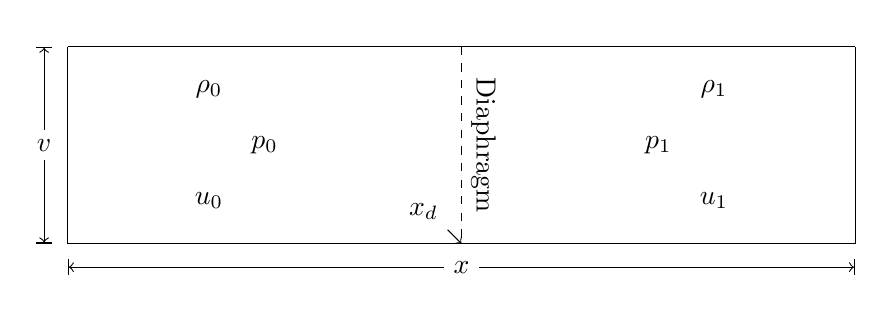
\begin{tikzpicture}
% place nodes
\node[] at (0, 0) (a) {};
\node[] at (0,-.3) (a1){};
\node[] at (-.3,0) (a2){};
\node[] at (10,0) (b) {};
\node[] at (10,-.3) (b1){};

\node[] at (0,2.5)  (c) {};
\node[] at (-.3,2.5) (c1){};
\node[] at (10,2.5) (d) {};

\node[] at (5,2.5)  (e) {};
\node[] at (5,0) (f) {};

% draw edges  
\draw[] (a.center) -- (b.center) {};
\draw[|<->|] (a1.center) -- (b1.center) node[midway,fill=white] (TextNode) {\(x\)};
\draw[] (a.center) -- (c.center) {};
\draw[|<->|] (a2.center) -- (c1.center) node[midway,fill=white] (TextNode) {\(v\)};
\draw[] (c.center) -- (d.center) node[above] {};
\draw[] (d.center) -- (b.center) node[above] {};
\draw[dashed] (e.center) -- (f.center) node[sloped,above,midway] {Diaphragm};
\draw[<-] (f.center)-- +(-5pt,5pt) node[above left] {\(x_d\)};

%draw quantities
\node[] at (2.5,1.25) (T){\(p_0\)};
\node [above left of=T] (rho) {\(\rho_0\)}; 
\node [below left of=T] (v) {\(u_0\)};

\node[] at (7.5,1.25) (T0){\(p_1\)};
\node [above right of=T0] (rho0) {\(\rho_1\)}; 
\node [below right of=T0] (v0) {\(u_1\)};
\end{tikzpicture}
	\caption{Problem setup for Sod's shock tube in 1D translated for the BGK model in velocity \(v\) and space \(x\). A diaphragm is positioned at \(x_d\), seperating the whole domain in two regions (region 1 and region 5). Initial conditions for density \(\rho\), pressure \(p\) and macroscopic velocity \(u\) are indicated.}
	\label{Fig:SodProbSetup}
\end{figure}
At \(t>0\) the diaphragm is broken, which leads to the formation of five regions which are depicted in \cref{Fig:SodTime0}. Between \(x_1\) and \(x_2\) we find the head and tail of the rarefaction wave traveling left. The solution for \(\rho\), \(p\) and \(u\) is continuous in this area. The rarefaction wave is clearly discernible for a dilution of \(\Kn=0.01\) and \(\Kn=0.00001\) as seen \cref{Fig:SODHyRare}. The contact discontinuity at \(x_3\) is the point where a particle traveled from it's initial location at \(x_d\) in a time \(\Delta t\). The original paper by Sod mentions here, that across the contact discontinuity \(x_3\) the macroscopic velocity \(u\) and the pressure \(p\) are continuous in  contrast to the density \(\rho\) and the energy \(E\), as depicted in \cref{Fig:SodTime0}. This cannot be assumed for rarefied gases with \(\Kn=0.01\) as seen in \cref{Fig:SODHyRare}. A pronounced contact discontinuity in the density \(\rho\) and the energy \(E\) cannot be found. Labeled as \(x_4\) is the position of the shock wave, at which in general none of the microscopic quantities will be continuous for gases with \(\Kn=0.00001\). Again this does not hold for rarefied regimes as seen in \cref{Fig:SODHyRare}.\\
Note, that \cref{Fig:SodTime} and \cref{Fig:SodTime0} is taken from \cite{Sod} in order to elaborate the general evolution in time of a gas of \(\Kn<0.01\) in Sod's shock tube. \Cref{Fig:ExamplesSod} shows solutions \(f(t_i,v,x)\) of the BGK model with \(t_0=0s\),\(t_1=0.06\) and \(t_3=0.12s\) for two rarefaction levels \(\Kn=0.00001\) and \(\Kn=0.01\). There the difference when increasing the dilution of a gas in Sod's shock tube is visible: An increased dilution leads to a smooth transition from region 1 to region 5 with the abundance of a pronounced shock front. 
\begin{figure}[H]
	\begin{subfigure}{.45\textwidth}
		\centering
		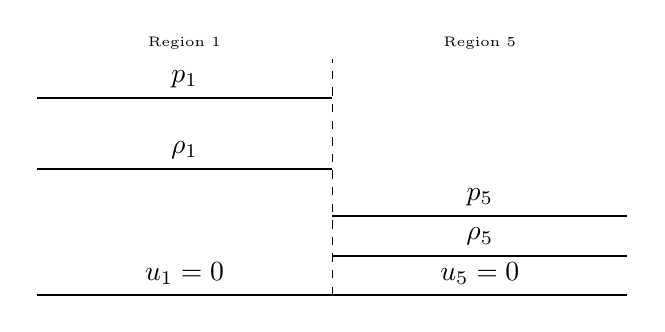
\begin{tikzpicture}
		%ground nodes
	\node [] at (0,0) (a0) {};
	\node [] at (3.75,0) (a3) {};
	\node [] at (7.5,0) (a6) {};
		%level 1 nodes
	\node [] at (0,1.6) (f0) {};
	\node [] at (3.75,1.6) (f1) {};
	\node [] at (7.5,0.5) (b6) {};
	
		%level 2 nodes
	\node [] at (0,2.5) (h0) {};
	\node [] at (3.75,2.5) (h1) {};
	\node [] at (3.75,0.5) (b3) {};
	\node [] at (7.5,1) (d6) {};
	\node [] at (3.75,1) (d3) {};	
		%top nodes
	\node [] at (0,3) (i0) {};
	\node [] at (3.75,3) (i3) {};
	\node [] at (7.5,3) (i6) {};
	
	\draw[thick] (a0.center) -- (a3.center) node [midway,above] {$u_1=0$};
	\draw[thick] (f0.center) -- (f1.center) node [midway,above] {$\rho_1$};
	\draw[thick] (h0.center) -- (h1.center) node [midway,above] {$p_1$};
	
	\draw[thick] (a3.center) -- (a6.center) node [midway,above] { $u_5=0$};
	\draw[thick] (b3.center) -- (b6.center) node [midway,above] {$\rho_5$};
	\draw[thick] (d3.center) -- (d6.center) node [midway,above] {$p_5$};
	\draw[dashed] (a3.center) -- (i3.center) {};
	\path[] (i0.center) -- (i3.center) node [midway,above] {\tiny Region 1};
	\path[] (i3.center) -- (i6.center) node [midway,above] {\tiny Region 5};
\end{tikzpicture}
		\caption{Sod's shock tube at \(t=0\). The whole domain is split into two regions with corresponding initial conditions for pressure \(p\), density \(\rho\) and macroscopic velocity \(u\). Position of the diaphragm is labeled as \(x_d\).\\ \\ \\}
		\label{Fig:SodTime}
	\end{subfigure}\hfill
	\begin{subfigure}{.45\textwidth}
		\centering
		\begin{tikzpicture}
	%ground nodes
	\node [] at (0,0) (a0) {};
	\node [] at (2,0) (a1) {};
	\node [] at (3,0) (a2) {};
	\node [] at (3.5,0) (a3) {};
	\node [] at (4.5,0) (a4) {};
	\node [] at (5.5,0) (a5) {};
	\node [] at (7.5,0) (a6) {};
	\node [on grid,below = 1.5ex of a2] (xd) {$x_d$};
	\node [on grid,below = 1.5ex of a1] (x1) {$x_1$};
	\node [on grid,below = 1.5ex of a3] (x2) {$x_2$};
	\node [on grid,below = 1.5ex of a4] (x3) {$x_3$};
	\node [on grid,below = 1.5ex of a5] (x4) {$x_4$};
	%level 1 nodes
	\node [] at (7.5,0.5) (b6) {};
	\node [] at (5.5,0.5) (b5) {};
	%level 2 nodes
	\node [] at (3,.9) (c2) {};
	\node [] at (3.5,.9) (c3) {};
	\node [] at (4.5,.9) (c4) {};
	%level 3 nodes
	\node [] at (7.5,1) (d6) {};
	\node [] at (5.5,1) (d5) {};
	%level 4 nodes
	\node [] at (4.5,1.5) (e4) {};
	\node [] at (5.5,1.5) (e5) {};
	%level 5 nodes
	\node [] at (0,1.6) (f0) {};
	\node [] at (2,1.6) (f1) {};
	%level 6 nodes
	\node [] at (3,2) (g2) {};
	\node [] at (3.5,2) (g3) {};
	\node [] at (4.5,2) (g4) {};
	\node [] at (5.5,2) (g5) {};
	\node [] at (7.5,2) (g6) {};
	%level 7 nodes
	\node [] at (0,2.5) (h0) {};
	\node [] at (2,2.5) (h1) {};
	\node [] at (3,2.5) (h2) {};
	\node [] at (3.5,2.5) (h3) {};
	\node [] at (4.5,2.5) (h4) {};
	\node [] at (5.5,2.5) (h5) {};
	%top nodes
	\node [] at (0,3) (i0) {};
	\node [] at (2,3) (i1) {};
	\node [] at (3,3) (i2) {};
	\node [] at (3.5,3) (i3) {};
	\node [] at (4.5,3) (i4) {};
	\node [] at (5.5,3) (i5) {};
	\node [] at (7.5,3) (i6) {};
	%draw and bottom edge
	\draw [|->,thick] (a0.center) -- (a6.center) node [below left] {$x$};
	\path [] (a0.center) -- (a1.center) node [midway,above] {$u_1$};
	\path [] (a5.center) -- (a6.center) node [midway,above] { $u_5$};
	%draw top descriptors
	\path[] (i0.center) -- (i1.center) node [midway,above] {\tiny Region 1};
	\path[] (i1.center) -- (i3.center) node [midway,above] {\tiny Region 2};
	\path[] (i3.center) -- (i4.center) node [midway,above] {\tiny Reg.3};
	\path[] (i4.center) -- (i5.center) node [midway,above] {\tiny Reg.4};
	\path[] (i5.center) -- (i6.center) node [midway,above] {\tiny Region 5};
	%draw level 1
	\draw[thick] (b5.center) -- (b6.center) {};
	\path[] (b5.center) -- (b6.center) node [midway,above] {$\rho_5$};
	%draw level 3
	\path[] (c3.center) -- (c4.center) node [midway,above] {$\rho_3$};
	%draw level 4
	\draw[thick] (d5.center) -- (d6.center) {};
	\path[] (d5.center) -- (d6.center) node [midway,above] {$p_5$};
	%draw level 5
	\draw[thick] (e4.center) -- (e5.center) {};
	\path[] (e4.center) -- (e5.center) node [midway,above] {$\rho_4$};
	\draw[thick] plot [smooth] coordinates {(f1)(2.6,1.1)(c2)(c3)(c4)};
	\draw[thick] (f0.center) -- (f1.center) node [midway,above] {$\rho_1$};
	%draw level 6
	\path[] (g3.center) -- (g4.center) node [midway,above] {$p_3$};
	\path[] (g4.center) -- (g5.center) node [midway,above] {$p_4$};
	\draw[thick] plot [smooth] coordinates {(h1)(2.5,2.2)(g2)(g3)(g4)(g5)};
	\draw[thick] (h3.center) -- (a1.center) {};

	\draw[thick] (h0.center) -- (h1.center) node [midway,above] {$p_1$};
	\draw[thick] (h3.center) -- (h4.center) node [midway,above] {$u_3$};
	\draw[thick] (h4.center) -- (h5.center) node [midway,above] {$u_4$};
	%draw vertical lines
	\draw[dashed] (a1.center) -- (i1.center) {};
	\draw[dashed] (a2.center) -- (h2.center) {};
	\draw[dashed] (a3.center) -- (i3.center) {};
	\draw[dashed] (a4.center) -- (i4.center) {};
	\draw[dashed] (a5.center) -- (i5.center) {};

\end{tikzpicture}
		\caption{Sod's shock tube at \(t>0\). Shown are pressure \(p\), denisty \(\rho\)  and macroscoppic velocity \(u\). Five regions can be identified marked out with \(x_1\) and \(x_2\) as head and tail of the rarefaction wave, \(x_3\) as the contact discontinuity and \(x_4\) as the position of the shock wave. The position of the initial diaphragm is labeled \(x_d\). A particle that traveled from \(x_d\) during \(\Delta t\) will be located at \(x_3\).}
		\label{Fig:SodTime0}
	\end{subfigure}\\ \vfill
	\begin{subfigure}{\textwidth}
		\centering
		\input{Figures/BGK/ExamplesSod.tex}
		\vspace{-10pt}
		\caption{Two solutions of the BGK model \(f(t_i,v,x)\) in Sod's shock tube with \(\Kn=0.00001\) (top row) and \(\Kn=0.01\) (bottom row) for a fixed time \(t_i\). Solutions are presented for \(t_0=0s\), \(t_1=0.06s\) and \(t_2=0.12s\).}
		\label{Fig:ExamplesSod}
	\end{subfigure}\\%\vspace{5pt}
	\begin{subfigure}{\textwidth}
		% This file was created by tikzplotlib v0.9.6.
\begin{tikzpicture}

\begin{groupplot}[group style={group size=3 by 1,horizontal sep=1.5cm}]
\nextgroupplot[
legend cell align={left},
legend style={fill opacity=0.1, draw opacity=1, text opacity=1, draw=none},
tick align=outside,
tick pos=left,
x grid style={white!69.0196078431373!black},
xlabel={\(x\)},
xmin=-0.04725, xmax=1.04725,
xtick style={color=black},
xtick={0,0.2525,0.48,0.61,0.75,1},
xticklabels={0,$x_1$,$x_2$,$x_3$,$x_4$,1},
y grid style={white!69.0196078431373!black},
ylabel={\(\rho\)},
ymin=0.0812472272613489, ymax=1.04375013203517,
ytick style={color=black},
ytick={0,0.2,0.4,0.6,0.8,1,1.2},
yticklabels={0.0,0.2,0.4,0.6,0.8,1.0,1.2},
width=.33\textwidth,
height=.25\textwidth
]
\addplot [semithick, color0, mark=o,mark repeat=25,mark repeat=20,mark size=1.5pt]
table {%
0.0025 0.999999999999998
0.0075 0.999999999999989
0.0125 0.999999999999973
0.0175 0.999999999999938
0.0225 0.999999999999854
0.0275 0.999999999999657
0.0325 0.999999999999225
0.0375 0.999999999998307
0.0425 0.999999999996346
0.0475 0.999999999992153
0.0525 0.999999999983302
0.0575 0.999999999964812
0.0625 0.999999999926618
0.0675 0.999999999848593
0.0725 0.999999999691032
0.0775 0.999999999376523
0.0825 0.999999998755951
0.0875 0.999999997545765
0.0925 0.999999995213722
0.0975 0.999999990773699
0.1025 0.999999982422727
0.1075 0.999999966908873
0.1125 0.999999938447061
0.1175 0.999999886889466
0.1225 0.999999794688685
0.1275 0.999999631942622
0.1325 0.999999348451367
0.1375 0.999998861215854
0.1425 0.99999803513588
0.1475 0.999996653797842
0.1525 0.999994376182765
0.1575 0.999990673914891
0.1625 0.999984742419316
0.1675 0.999975378267931
0.1725 0.999960814384862
0.1775 0.999938505100111
0.1825 0.999904854832319
0.1875 0.999854888023955
0.1925 0.99978186432473
0.1975 0.999676852094109
0.2025 0.9995282847065
0.2075 0.999321536763255
0.2125 0.999038569143143
0.2175 0.998657700112069
0.2225 0.998153561405535
0.2275 0.997497290690344
0.2325 0.996656993873317
0.2375 0.99559848331206
0.2425 0.994286264568487
0.2475 0.992684710498992
0.2525 0.990759333664029
0.2575 0.988478051967666
0.2625 0.98581234145918
0.2675 0.982738184425117
0.2725 0.979236747133095
0.2775 0.975294754490673
0.2825 0.970904562368228
0.2875 0.966063957098391
0.2925 0.960775732208377
0.2975 0.955047103436866
0.3025 0.948889025126006
0.3075 0.942315466055067
0.3125 0.935342693163985
0.3175 0.927988599833952
0.3225 0.920272103437352
0.3275 0.912212626120219
0.3325 0.903829663999579
0.3375 0.895142443413195
0.3425 0.886169658461554
0.3475 0.876929281542178
0.3525 0.867438437521144
0.3575 0.857713332238945
0.3625 0.847769226883468
0.3675 0.837620451126894
0.3725 0.827280449648232
0.3775 0.816761858656435
0.3825 0.806076611284112
0.3875 0.795236073302906
0.3925 0.784251213671778
0.3975 0.773132818216759
0.4025 0.761891759626233
0.4075 0.750539343464475
0.4125 0.739087758804205
0.4175 0.727550674370907
0.4225 0.715944038086624
0.4275 0.704287161112698
0.4325 0.692604198229712
0.4375 0.680926174533778
0.4425 0.669293749303168
0.4475 0.657760935139416
0.4525 0.646399961099968
0.4575 0.635307285171405
0.4625 0.62461023214634
0.4675 0.614472547467368
0.4725 0.605094999885858
0.4775 0.596704255186181
0.4825 0.58952161507939
0.4875 0.583707951716951
0.4925 0.579297599755217
0.4975 0.576156316434373
0.5025 0.574000969056694
0.5075 0.572480179189811
0.5125 0.571264203656635
0.5175 0.570086382765471
0.5225 0.568721460109119
0.5275 0.566925165174661
0.5325 0.564365792996614
0.5375 0.560570509046267
0.5425 0.554906055797055
0.5475 0.546613499580239
0.5525 0.534908971753206
0.5575 0.51914228036301
0.5625 0.498978621789052
0.5675 0.474548680779275
0.5725 0.446512149382244
0.5775 0.416003356002158
0.5825 0.384466862363659
0.5875 0.35342828965285
0.5925 0.324264603478363
0.5975 0.298031575214768
0.6025 0.275379774683857
0.6075 0.25655829783077
0.6125 0.241481617940157
0.6175 0.229826469375018
0.6225 0.221130574377751
0.6275 0.214876145355647
0.6325 0.210551637309679
0.6375 0.207691967900792
0.6425 0.205900479181207
0.6475 0.204856774754392
0.6525 0.204314508374631
0.6575 0.204092813817174
0.6625 0.204064484192581
0.6675 0.204143252251004
0.6725 0.204271660594381
0.6775 0.204410149561804
0.6825 0.204527209819603
0.6875 0.2045897518297
0.6925 0.204552165643129
0.6975 0.204341777937618
0.7025 0.203837534924661
0.7075 0.202838126194388
0.7125 0.201017076265398
0.7175 0.197870634170907
0.7225 0.192691647141719
0.7275 0.184667360813301
0.7325 0.173289806057922
0.7375 0.159203831239715
0.7425 0.144954929560638
0.7475 0.134090936270534
0.7525 0.128237751279186
0.7575 0.125970039515887
0.7625 0.125265822009891
0.7675 0.125069122324036
0.7725 0.125016332608434
0.7775 0.125002354962472
0.7825 0.12499867180924
0.7875 0.124997703549099
0.7925 0.124997449439354
0.7975 0.124997382859364
0.8025 0.12499736544419
0.8075 0.124997360897239
0.8125 0.124997359712403
0.8175 0.124997359404317
0.8225 0.124997359324391
0.8275 0.124997359303707
0.8325 0.124997359298369
0.8375 0.124997359296995
0.8425 0.124997359296643
0.8475 0.124997359296553
0.8525 0.12499735929653
0.8575 0.124997359296525
0.8625 0.124997359296523
0.8675 0.124997359296523
0.8725 0.124997359296523
0.8775 0.124997359296523
0.8825 0.124997359296523
0.8875 0.124997359296523
0.8925 0.124997359296523
0.8975 0.124997359296523
0.9025 0.124997359296523
0.9075 0.124997359296523
0.9125 0.124997359296523
0.9175 0.124997359296523
0.9225 0.124997359296523
0.9275 0.124997359296523
0.9325 0.124997359296523
0.9375 0.124997359296523
0.9425 0.124997359296523
0.9475 0.124997359296523
0.9525 0.124997359296523
0.9575 0.124997359296523
0.9625 0.124997359296523
0.9675 0.124997359296523
0.9725 0.124997359296523
0.9775 0.124997359296523
0.9825 0.124997359296523
0.9875 0.124997359296523
0.9925 0.124997359296523
0.9975 0.124997359296523
};
\addlegendentry{\small \(\hy\)}
\addplot [semithick, red, mark=square,mark repeat=20,mark size=1pt]
table {%
0.0025 0.99999981316608
0.0075 0.99999975421908
0.0125 0.999999680296827
0.0175 0.999999584015259
0.0225 0.999999457570282
0.0275 0.999999291316442
0.0325 0.999999072816931
0.0375 0.999998785865599
0.0425 0.999998409307099
0.0475 0.999997915549681
0.0525 0.999997268671227
0.0575 0.999996422006429
0.0625 0.999995315081933
0.0675 0.999993869739663
0.0725 0.999991985257259
0.0775 0.999989532239156
0.0825 0.999986345012926
0.0875 0.999982212224108
0.0925 0.999976865280456
0.0975 0.999969964255601
0.1025 0.999961080825805
0.1075 0.999949677785936
0.1125 0.999935084677325
0.1175 0.999916469067197
0.1225 0.999892803054168
0.1275 0.999862824644981
0.1325 0.999824993762287
0.1375 0.999777442809534
0.1425 0.99971792194299
0.1475 0.999643739485772
0.1525 0.999551698263626
0.1575 0.999438029040718
0.1625 0.999298322672216
0.1675 0.999127463048146
0.1725 0.998919563350529
0.1775 0.998667908546717
0.1825 0.998364907354493
0.1875 0.998002057094462
0.1925 0.997569924850764
0.1975 0.997058148157106
0.2025 0.996455457989507
0.2075 0.995749726175553
0.2125 0.994928038439235
0.2175 0.993976793230499
0.2225 0.992881825300824
0.2275 0.991628551759091
0.2325 0.990202137164675
0.2375 0.988587673176978
0.2425 0.986770367464113
0.2475 0.984735736041917
0.2525 0.982469793006896
0.2575 0.979959231754083
0.2625 0.977191592215162
0.2675 0.974155409371525
0.2725 0.970840339230837
0.2775 0.967237259535191
0.2825 0.963338343623945
0.2875 0.959137107042427
0.2925 0.954628427617574
0.2975 0.949808540774016
0.3025 0.944675012808809
0.3075 0.939226695650786
0.3125 0.93346366726498
0.3175 0.927387162272547
0.3225 0.920999497473236
0.3275 0.914303996700869
0.3325 0.907304918741389
0.3375 0.90000739086861
0.3425 0.89241734896415
0.3475 0.884541483383983
0.3525 0.876387188096097
0.3575 0.867962509719168
0.3625 0.859276093668592
0.3675 0.850337127400342
0.3725 0.841155286214046
0.3775 0.831740695052687
0.3825 0.822103928898359
0.3875 0.812256081874584
0.3925 0.802208936708843
0.3975 0.79197525683824
0.4025 0.78156919951702
0.4075 0.771006810236054
0.4125 0.760306513523842
0.4175 0.749489476246309
0.4225 0.738579702514359
0.4275 0.727603733467464
0.4325 0.716589865685254
0.4375 0.705566854549949
0.4425 0.694562138954764
0.4475 0.683599784307639
0.4525 0.672698744484615
0.4575 0.661872778856293
0.4625 0.651134054393569
0.4675 0.640501846359315
0.4725 0.630014077905235
0.4775 0.619732885281825
0.4825 0.60973151025046
0.4875 0.600058308646607
0.4925 0.590696148720204
0.4975 0.581551386384131
0.5025 0.572476510359754
0.5075 0.563293926378223
0.5125 0.553800236231206
0.5175 0.543781524364539
0.5225 0.533063510452134
0.5275 0.521566257579677
0.5325 0.509313962288544
0.5375 0.496400822236544
0.5425 0.482943372019684
0.5475 0.469048302365069
0.5525 0.454804360618456
0.5575 0.440289849071466
0.5625 0.425583491928963
0.5675 0.41077164651714
0.5725 0.395950814468977
0.5775 0.381227050612487
0.5825 0.366713604395908
0.5875 0.352527021957449
0.5925 0.338781439243636
0.5975 0.325581204566807
0.6025 0.313012828321206
0.6075 0.301137932019271
0.6125 0.289988932118549
0.6175 0.279568586970621
0.6225 0.269853520854869
0.6275 0.26080082760768
0.6325 0.252356199651869
0.6375 0.244461884500335
0.6425 0.237063086804866
0.6475 0.230112021380132
0.6525 0.223569464145314
0.6575 0.217404176438371
0.6625 0.211590906449739
0.6675 0.206107783930591
0.6725 0.200933852741061
0.6775 0.19604728678763
0.6825 0.191424573503377
0.6875 0.187040687492616
0.6925 0.182870065685786
0.6975 0.17888806575569
0.7025 0.175072550584356
0.7075 0.171405281352616
0.7125 0.167872894069909
0.7175 0.164467347431299
0.7225 0.161185835445557
0.7275 0.158030237217974
0.7325 0.155006220934256
0.7375 0.152122132077785
0.7425 0.149387786605452
0.7475 0.146813269947481
0.7525 0.144407822244173
0.7575 0.142178874538462
0.7625 0.140131289623276
0.7675 0.138266850742206
0.7725 0.136584026151337
0.7775 0.135078014784042
0.7825 0.133741049493288
0.7875 0.132562905381218
0.7925 0.131531539089185
0.7975 0.130633776435876
0.8025 0.129855972071242
0.8075 0.129184582884318
0.8125 0.128606620847313
0.8175 0.128109974484943
0.8225 0.12768360662565
0.8275 0.127317647528726
0.8325 0.127003407220149
0.8375 0.126733330622757
0.8425 0.126500915923433
0.8475 0.126300612357069
0.8525 0.126127709374185
0.8575 0.125978225574316
0.8625 0.125848802984529
0.8675 0.125736610164789
0.8725 0.125639256072876
0.8775 0.12555471547341
0.8825 0.125481265823031
0.8875 0.125417434945145
0.8925 0.125361958389225
0.8975 0.125313745129744
0.9025 0.125271850176076
0.9075 0.125235452709076
0.9125 0.125203838498512
0.9175 0.125176385551639
0.9225 0.125152552162449
0.9275 0.125131866744975
0.9325 0.125113919022193
0.9375 0.125098352293426
0.9425 0.125084856614912
0.9475 0.12507316280418
0.9525 0.125063037227494
0.9575 0.125054277361622
0.9625 0.125046708146471
0.9675 0.125040179165499
0.9725 0.125034562672888
0.9775 0.125029752262378
0.9825 0.125025660897079
0.9875 0.125022212914257
0.9925 0.12501931099985
0.9975 0.125016719545722
};
\addlegendentry{\small \(\rare\)}
\addplot [semithick,dashed]
table {%
0.2525 0
0.2525 1.5
};
\addplot [semithick,dashed]
table {%
	0.48 0
	0.48 1.5
};
\addplot [semithick,dashed]
table {%
	0.61 0
	0.61 1.5
};
\addplot [semithick,dashed]
table {%
	0.75 0
	0.75 1.5
};
\nextgroupplot[
legend cell align={left},
legend style={fill opacity=0.1, draw opacity=1, text opacity=1,draw=none},
tick align=outside,
tick pos=left,
x grid style={white!69.0196078431373!black},
xlabel={\(x\)},
xmin=-0.04725, xmax=1.04725,
xtick style={color=black},
xtick={0,0.2525,0.48,0.61,0.75,1},
xticklabels={0,$x_1$,$x_2$,$x_3$,$x_4$,1},
y grid style={white!69.0196078431373!black},
ylabel={\(\rho u\)},
ymin=-0.0207805766857379, ymax=0.436392110400496,
ytick style={color=black},
ytick={-0.1,0,0.1,0.2,0.3,0.4,0.5},
yticklabels={−0.1,0.0,0.1,0.2,0.3,0.4,0.5},
width=.33\textwidth,
height=.25\textwidth
]
\addplot [semithick, color0, mark=o,mark repeat=25,mark repeat=20,mark size=1.5pt]
table {%
0.0025 6.30909942701128e-15
0.0075 2.52743810784534e-14
0.0125 6.71665952599217e-14
0.0175 1.47797315819247e-13
0.0225 3.07924884094236e-13
0.0275 6.61724731226376e-13
0.0325 1.42564590793223e-12
0.0375 3.07415836396623e-12
0.0425 6.61513600596091e-12
0.0475 1.41586576150479e-11
0.0525 3.00685205419515e-11
0.0575 6.32804201327425e-11
0.0625 1.3184036970615e-10
0.0675 2.71816269673475e-10
0.0725 5.54376851469977e-10
0.0775 1.11825149908461e-09
0.0825 2.23051509342037e-09
0.0875 4.39884368497434e-09
0.0925 8.5758772306255e-09
0.0975 1.65259662279758e-08
0.1025 3.14735318416989e-08
0.1075 5.92319223420021e-08
0.1125 1.10138321629211e-07
0.1175 2.02317178115227e-07
0.1225 3.67093738893431e-07
0.1275 6.57821443877529e-07
0.1325 1.16402288185517e-06
0.1375 2.03362897054613e-06
0.1425 3.50728901639945e-06
0.1475 5.97025142461952e-06
0.1525 1.00291759427997e-05
0.1575 1.66233527041188e-05
0.1625 2.71819700399184e-05
0.1675 4.38409224509142e-05
0.1725 6.97336019227715e-05
0.1775 0.000109369363494647
0.1825 0.000169109905168177
0.1875 0.000257746596586162
0.1925 0.000387169951738958
0.1975 0.000573105629364502
0.2025 0.00083587020550754
0.2075 0.00120107655052603
0.2125 0.00170019665307498
0.2175 0.00237087432492865
0.2225 0.0032568772432988
0.2275 0.00440759238754277
0.2325 0.00587700375526764
0.2375 0.00772214479508426
0.2425 0.0100010837905844
0.2475 0.0127705676361399
0.2525 0.0160835050774659
0.2575 0.0199865027249069
0.2625 0.0245176686528201
0.2675 0.0297048684855691
0.2725 0.0355645636560769
0.2775 0.0421012920749302
0.2825 0.0493077806620858
0.2875 0.0571656185418088
0.2925 0.065646376882973
0.2975 0.074713039379489
0.3025 0.0843216049455656
0.3075 0.0944227371486421
0.3125 0.10496335769442
0.3175 0.115888108463717
0.3225 0.127140633730189
0.3275 0.138664658219507
0.3325 0.150404855967261
0.3375 0.162307519006456
0.3425 0.17432104407487
0.3475 0.186396260539237
0.3525 0.198486624527203
0.3575 0.210548303768142
0.3625 0.222540175680823
0.3675 0.234423758453756
0.3725 0.246163091716497
0.3775 0.257724580217212
0.3825 0.269076810899138
0.3875 0.280190351007068
0.3925 0.291037532389737
0.3975 0.301592224987379
0.4025 0.311829600578427
0.4075 0.32172588617664
0.4125 0.33125810501847
0.4175 0.340403801924414
0.4225 0.349140749159004
0.4275 0.357446629223257
0.4325 0.365298693275803
0.4375 0.372673400036284
0.4425 0.379546053737188
0.4475 0.385890487528712
0.4525 0.391678891683233
0.4575 0.396881980082096
0.4625 0.40146984092481
0.4675 0.405414027071735
0.4725 0.408691633111172
0.4775 0.411292026446267
0.4825 0.413226031432564
0.4875 0.414535188150287
0.4925 0.415295778738166
0.4975 0.415611533714758
0.5025 0.415593775426746
0.5075 0.415336272676748
0.5125 0.414895448502171
0.5175 0.414279737593578
0.5225 0.413441915625134
0.5275 0.412265559121292
0.5325 0.410543071971494
0.5375 0.407952686344571
0.5425 0.404050222699679
0.5475 0.398294145414728
0.5525 0.390116261831736
0.5575 0.379034708912469
0.5625 0.364785477913794
0.5675 0.347433285813965
0.5725 0.327421674382695
0.5775 0.305538967700042
0.5825 0.282804901002568
0.5875 0.260309644556986
0.5925 0.239050562602313
0.5975 0.21980754302411
0.6025 0.203079346386846
0.6075 0.189081108100233
0.6125 0.177786617803809
0.6175 0.168993000834794
0.6225 0.162388542023055
0.6275 0.157611733202854
0.6325 0.15429658772856
0.6375 0.152103712729153
0.6425 0.150738704834072
0.6475 0.149960168581477
0.6525 0.149579859369824
0.6575 0.149457422785557
0.6625 0.149491944246978
0.6675 0.149612013943466
0.6725 0.14976530020989
0.6775 0.149907791760532
0.6825 0.14999195731766
0.6875 0.14995203609554
0.6925 0.149683391775078
0.6975 0.149011229469267
0.7025 0.147642220299706
0.7075 0.145092234771363
0.7125 0.140589880897931
0.7175 0.132983874719494
0.7225 0.12076396568901
0.7275 0.102471387896822
0.7325 0.0779153049527428
0.7375 0.0500927747148544
0.7425 0.0255869635272696
0.7475 0.0101029770633572
0.7525 0.00323067179465287
0.7575 0.000916685484344893
0.7625 0.000247535673412993
0.7675 6.57015398035193e-05
0.7725 1.73347678877712e-05
0.7775 4.56166544163445e-06
0.7825 1.19832317827514e-06
0.7875 3.14296212372224e-07
0.7925 8.22998347460696e-08
0.7975 2.15132337412575e-08
0.8025 5.61307173932267e-09
0.8075 1.46156536596175e-09
0.8125 3.79741252383841e-10
0.8175 9.84313849249286e-11
0.8225 2.54493090390674e-11
0.8275 6.56196973336829e-12
0.8325 1.68704997701825e-12
0.8375 4.32438917614844e-13
0.8425 1.10497771029924e-13
0.8475 2.81771756164485e-14
0.8525 7.1446327166275e-15
0.8575 1.78835623869184e-15
0.8625 4.08881037663235e-16
0.8675 5.2382325353727e-17
0.8725 2.23070013203397e-18
0.8775 -1.70270270785549e-18
0.8825 1.91820140579613e-19
0.8875 -2.40410876608015e-18
0.8925 -2.60371401563257e-18
0.8975 1.34734438717905e-19
0.9025 1.35175634880655e-19
0.9075 1.35610010757515e-19
0.9125 1.35610010757515e-19
0.9175 1.35610010757515e-19
0.9225 1.35610010757515e-19
0.9275 1.35610010757515e-19
0.9325 1.35610010757515e-19
0.9375 1.35610010757515e-19
0.9425 1.35610010757515e-19
0.9475 1.35610010757515e-19
0.9525 1.35610010757515e-19
0.9575 1.35610010757515e-19
0.9625 1.35610010757515e-19
0.9675 1.35610010757515e-19
0.9725 1.35610010757515e-19
0.9775 1.35610010757515e-19
0.9825 1.35610010757515e-19
0.9875 1.35610010757515e-19
0.9925 1.35610010757515e-19
0.9975 1.35610010757515e-19
};
\addlegendentry{\small \(\hy\)}
\addplot [semithick, red, mark=square,mark repeat=20,mark size=1pt]
table {%
0.0025 4.54455299100046e-07
0.0075 5.99854726306051e-07
0.0125 7.8833937943175e-07
0.0175 1.03258649420672e-06
0.0225 1.34970552357957e-06
0.0275 1.76218162719785e-06
0.0325 2.29933730512723e-06
0.0375 2.9993028510072e-06
0.0425 3.91157902756794e-06
0.0475 5.10032659340901e-06
0.0525 6.64856011169223e-06
0.0575 8.66346749193427e-06
0.0625 1.1283125362535e-05
0.0675 1.46849349680372e-05
0.0725 1.90961639813164e-05
0.0775 2.48070458569648e-05
0.0825 3.21869585645296e-05
0.0875 4.17042761626466e-05
0.0925 5.39505557152346e-05
0.0975 6.96697830363863e-05
0.1025 8.97934463024172e-05
0.1075 0.000115482227362561
0.1125 0.00014817508525939
0.1175 0.00018964644172765
0.1225 0.000242072049645008
0.1275 0.000308103917080716
0.1325 0.000390954356975003
0.1375 0.000494488822951434
0.1425 0.000623326667101406
0.1475 0.000782948314726992
0.1525 0.000979806602457875
0.1575 0.00122143919118749
0.1625 0.00151657807971254
0.1675 0.00187525136096786
0.1725 0.00230887154792676
0.1775 0.00283030413169527
0.1825 0.0034539096093941
0.1875 0.00419555212427541
0.1925 0.00507256817627539
0.1975 0.00610368964860908
0.2025 0.00730891668390221
0.2075 0.00870933771887943
0.2125 0.0103268961885164
0.2175 0.0121841059281862
0.2225 0.0143037199803669
0.2275 0.0167083601629121
0.2325 0.0194201171751697
0.2375 0.0224601330085379
0.2425 0.0258481788193049
0.2475 0.0296022420910958
0.2525 0.0337381368008472
0.2575 0.0382691494128088
0.2625 0.0432057319324069
0.2675 0.0485552510840276
0.2725 0.0543218001007408
0.2775 0.0605060768152644
0.2825 0.0671053289042067
0.2875 0.0741133644279057
0.2925 0.0815206233628243
0.2975 0.0893143037460852
0.3025 0.0974785344151436
0.3075 0.105994585179522
0.3125 0.11484110464153
0.3175 0.123994375817061
0.3225 0.133428580216276
0.3275 0.143116062129349
0.3325 0.153027586486912
0.3375 0.163132585720724
0.3425 0.173399393329266
0.3475 0.183795464026721
0.3525 0.194287581980226
0.3575 0.204842059214592
0.3625 0.215424925325016
0.3675 0.226002106937574
0.3725 0.236539591075874
0.3775 0.247003561570937
0.3825 0.257360493548
0.3875 0.26757719026068
0.3925 0.277620751863024
0.3975 0.287458479192157
0.4025 0.297057737197227
0.4075 0.306385828460686
0.4125 0.315409948964838
0.4175 0.324097304272163
0.4225 0.332415443906881
0.4275 0.340332821288337
0.4325 0.347819514440552
0.4375 0.35484796821436
0.4425 0.361393562340091
0.4475 0.367434779748903
0.4525 0.372952744621367
0.4575 0.377929946520065
0.4625 0.38234818701995
0.4675 0.386186388267707
0.4725 0.389419925219161
0.4775 0.392023892303592
0.4825 0.393981528311944
0.4875 0.395294661906065
0.4925 0.395987922268566
0.4975 0.396099555689399
0.5025 0.395658926713393
0.5075 0.394662325272313
0.5125 0.393063105985357
0.5175 0.390783106753753
0.5225 0.387738698310261
0.5275 0.383869352121223
0.5325 0.379155360021045
0.5375 0.373617300375614
0.5425 0.367302890237123
0.5475 0.360271900192528
0.5525 0.352586216657906
0.5575 0.344306227834089
0.5625 0.335491444318213
0.5675 0.326203075092749
0.5725 0.316507210045428
0.5775 0.306477788664165
0.5825 0.296198458188714
0.5875 0.285762282447909
0.5925 0.275268551155491
0.5975 0.264816737359117
0.6025 0.25449865135719
0.6075 0.244390587135066
0.6125 0.234547408729126
0.6175 0.225000011467603
0.6225 0.215756633727468
0.6275 0.206807461416989
0.6325 0.198131207855713
0.6375 0.189702055952046
0.6425 0.181495515904338
0.6475 0.173492239971993
0.6525 0.165679454368033
0.6575 0.158050244841829
0.6625 0.150601350337783
0.6675 0.143330323194121
0.6725 0.136232903033059
0.6775 0.129301264291135
0.6825 0.122523501442489
0.6875 0.115884390612929
0.6925 0.1093671852864
0.6975 0.102956019759651
0.7025 0.0966384287463818
0.7075 0.0904075357375704
0.7125 0.0842635839007025
0.7175 0.0782146386186505
0.7225 0.0722764400425698
0.7275 0.0664714991620224
0.7325 0.0608275999986637
0.7375 0.0553758968537104
0.7425 0.0501487924591837
0.7475 0.045177766924436
0.7525 0.0404913114022774
0.7575 0.0361131090887707
0.7625 0.0320605952695308
0.7675 0.0283440079834433
0.7725 0.0249660027875256
0.7775 0.0219218475058126
0.7825 0.0192001440166512
0.7875 0.0167839597388279
0.7925 0.0146522080278887
0.7975 0.0127811044806488
0.8025 0.0111455453501796
0.8075 0.00972029590602644
0.8125 0.00848092707308504
0.8175 0.00740448534503526
0.8225 0.00646991565985121
0.8275 0.00565827705059631
0.8325 0.00495279816714197
0.8375 0.00433881810166761
0.8425 0.00380365148512002
0.8475 0.00333640878221297
0.8525 0.00292779505335359
0.8575 0.00256990402128406
0.8625 0.00225601920638259
0.8675 0.00198042996503681
0.8725 0.00173826719329184
0.8775 0.00152536101752409
0.8825 0.00133812085700574
0.8875 0.00117343675845373
0.8925 0.00102859985494394
0.8975 0.00090123917588212
0.9025 0.000789271794310028
0.9075 0.000690863378432377
0.9125 0.000604396530399906
0.9175 0.00052844475296431
0.9225 0.000461750394540807
0.9275 0.000403205412331374
0.9325 0.000351834210560911
0.9375 0.000306778129286099
0.9425 0.000267281372367963
0.9475 0.000232678280462438
0.9525 0.000202381895071296
0.9575 0.000175873744959299
0.9625 0.000152694737618318
0.9675 0.00013243697449953
0.9725 0.000114736251193023
0.9775 9.92650033574736e-05
0.9825 8.57256827296962e-05
0.9875 7.38455370907372e-05
0.9925 6.33771043745151e-05
0.9975 5.41183398169117e-05
};
\addlegendentry{\small \(\rare\)}
\addplot [semithick,dashed]
table {%
	0.2525 0
	0.2525 1.5
};
\addplot [semithick,dashed]
table {%
	0.48 0
	0.48 1.5
};
\addplot [semithick,dashed]
table {%
	0.61 0
	0.61 1.5
};
\addplot [semithick,dashed]
table {%
	0.75 0
	0.75 1.5
};
\nextgroupplot[
legend cell align={left},
legend style={fill opacity=0.1, draw opacity=1, text opacity=1, draw=none},
tick align=outside,
tick pos=left,
x grid style={white!69.0196078431373!black},
xlabel={\(x\)},
xmin=-0.04725, xmax=1.04725,
xtick style={color=black},
xtick={0,0.2525,0.48,0.61,0.75,1},
xticklabels={0,$x_1$,$x_2$,$x_3$,$x_4$,1},
y grid style={white!69.0196078431373!black},
ylabel={\(E\)},
ymin=-0.01673310421985, ymax=1.02222538591518,
ytick style={color=black},
ytick={-0.2,0,0.2,0.4,0.6,0.8,1,1.2},
yticklabels={−0.2,0.0,0.2,0.4,0.6,0.8,1.0,1.2},
width=.33\textwidth,
height=.25\textwidth
]

\addplot [semithick, color0, mark=o,mark repeat=25,mark repeat=20,mark size=1.5pt]
table {%
0.0025 0.974999999999951
0.0075 0.974999999999907
0.0125 0.974999999999824
0.0175 0.974999999999669
0.0225 0.974999999999363
0.0275 0.974999999998719
0.0325 0.974999999997334
0.0375 0.974999999994361
0.0425 0.974999999988005
0.0475 0.97499999997449
0.0525 0.974999999946005
0.0575 0.974999999886615
0.0625 0.974999999764117
0.0675 0.974999999514247
0.0725 0.974999999010282
0.0775 0.974999998005467
0.0825 0.97499999602518
0.0875 0.974999992168127
0.0925 0.974999984744712
0.0975 0.974999970628869
0.1025 0.974999944113447
0.1075 0.974999894919787
0.1125 0.974999804790218
0.1175 0.974999641748242
0.1225 0.974999350589616
0.1275 0.974998837398088
0.1325 0.974997944775965
0.1375 0.974996412947483
0.1425 0.974993819843725
0.1475 0.974989490653573
0.1525 0.974982364144117
0.1575 0.974970799467683
0.1625 0.974952303544506
0.1675 0.974923156099602
0.1725 0.974877908067057
0.1775 0.974808730775096
0.1825 0.974704599839999
0.1875 0.974550310877258
0.1925 0.974325345523736
0.1975 0.974002636439099
0.2025 0.973547317759637
0.2075 0.972915589234677
0.2125 0.972053861336742
0.2175 0.970898375644783
0.2225 0.969375499011033
0.2275 0.967402861802382
0.2325 0.964891444638168
0.2375 0.96174861692709
0.2425 0.957882005938571
0.2475 0.953203947485006
0.2525 0.947636163508087
0.2575 0.941114251262602
0.2625 0.933591568377296
0.2675 0.925042159926081
0.2725 0.915462486128263
0.2775 0.904871850402083
0.2825 0.893311570998761
0.2875 0.880843061635519
0.2925 0.867545071311944
0.2975 0.853510374501746
0.3025 0.838842202878954
0.3075 0.823650677707796
0.3125 0.80804944992926
0.3175 0.792152694582577
0.3225 0.776072547066046
0.3275 0.759917017309144
0.3325 0.743788377532284
0.3375 0.727781990715895
0.3425 0.711985529261851
0.3475 0.696478524726255
0.3525 0.681332187714521
0.3575 0.666609439914812
0.3625 0.652365105973286
0.3675 0.638646220052745
0.3725 0.625492409437274
0.3775 0.61293632476802
0.3825 0.601004093017814
0.3875 0.589715774934755
0.3925 0.579085813345579
0.3975 0.569123462430903
0.4025 0.559833190932838
0.4075 0.551215054311751
0.4125 0.543265032207121
0.4175 0.535975328229931
0.4225 0.529334629143911
0.4275 0.523328319872161
0.4325 0.517938649476038
0.4375 0.513144841329374
0.4425 0.508923138416005
0.4475 0.505246772903584
0.4525 0.502085850252529
0.4575 0.499407147401467
0.4625 0.49717385201229
0.4675 0.495345329402208
0.4725 0.493877102148319
0.4775 0.492721325732655
0.4825 0.491827999856679
0.4875 0.49114676049528
0.4925 0.490628446577077
0.4975 0.490225574411412
0.5025 0.489892050726169
0.5075 0.489583251617593
0.5125 0.489255653552228
0.5175 0.488862480126186
0.5225 0.488342203004208
0.5275 0.487599742148386
0.5325 0.486483394633626
0.5375 0.484763982379149
0.5425 0.482126547018462
0.5475 0.478186641198099
0.5525 0.472539394541322
0.5575 0.464838905549125
0.5625 0.454891334433603
0.5675 0.44273416486432
0.5725 0.428673259277573
0.5775 0.413260856638999
0.5825 0.397217273102659
0.5875 0.381317978552166
0.5925 0.366277588773269
0.5975 0.35265968586857
0.6025 0.340828993937901
0.6075 0.33094700235995
0.6125 0.323000342106546
0.6175 0.316846468366913
0.6225 0.312262768652956
0.6275 0.308989979885994
0.6325 0.306765696589643
0.6375 0.305347195468759
0.6425 0.304524633083269
0.6475 0.30412640615635
0.6525 0.304018617899238
0.6575 0.3041004451537
0.6625 0.304296832802441
0.6675 0.304549364882103
0.6725 0.304805377771059
0.6775 0.305004369236508
0.6825 0.305059431344277
0.6875 0.304829615323252
0.6925 0.304076598389254
0.6975 0.302395775284873
0.7025 0.299109138529932
0.7075 0.293110237613966
0.7125 0.282676384199798
0.7175 0.265350695775959
0.7225 0.238216459608717
0.7275 0.199238534917943
0.7325 0.150286651533868
0.7375 0.100222394985358
0.7425 0.0619544979372982
0.7475 0.0414884570530703
0.7525 0.0337211704261632
0.7575 0.0313715712541428
0.7625 0.0307261916343882
0.7675 0.030554080991312
0.7725 0.030508566291402
0.7775 0.030496565798877
0.7825 0.030493407100338
0.7875 0.0304925768893975
0.7925 0.0304923590013502
0.7975 0.0304923019056265
0.8025 0.0304922869691739
0.8075 0.0304922830687958
0.8125 0.0304922820522722
0.8175 0.0304922817879033
0.8225 0.0304922817193052
0.8275 0.0304922817015494
0.8325 0.0304922816969657
0.8375 0.0304922816957857
0.8425 0.0304922816954828
0.8475 0.0304922816954053
0.8525 0.0304922816953855
0.8575 0.0304922816953805
0.8625 0.0304922816953792
0.8675 0.0304922816953787
0.8725 0.0304922816953786
0.8775 0.0304922816953786
0.8825 0.0304922816953786
0.8875 0.0304922816953786
0.8925 0.0304922816953786
0.8975 0.0304922816953786
0.9025 0.0304922816953786
0.9075 0.0304922816953786
0.9125 0.0304922816953786
0.9175 0.0304922816953786
0.9225 0.0304922816953786
0.9275 0.0304922816953786
0.9325 0.0304922816953786
0.9375 0.0304922816953786
0.9425 0.0304922816953786
0.9475 0.0304922816953786
0.9525 0.0304922816953786
0.9575 0.0304922816953786
0.9625 0.0304922816953786
0.9675 0.0304922816953786
0.9725 0.0304922816953786
0.9775 0.0304922816953786
0.9825 0.0304922816953786
0.9875 0.0304922816953786
0.9925 0.0304922816953786
0.9975 0.0304922816953786
};
\addlegendentry{\small \(\hy\)}
\addplot [semithick, red, mark=square,mark repeat=20,mark size=1pt]
table {%
0.0025 0.97499875113314
0.0075 0.974998415169894
0.0125 0.974997973548605
0.0175 0.974997395696738
0.0225 0.974996641899692
0.0275 0.974995660502251
0.0325 0.974994384412448
0.0375 0.974992726664499
0.0425 0.974990574773972
0.0475 0.974987783570467
0.0525 0.974984166129488
0.0575 0.974979482348512
0.0625 0.974973424623592
0.0675 0.974965599982967
0.0725 0.974955507924868
0.0775 0.974942513090756
0.0825 0.974925811787139
0.0875 0.974904391255565
0.0925 0.974876980490849
0.0975 0.974841991334292
0.1025 0.974797448537848
0.1075 0.974740907526093
0.1125 0.97466935869869
0.1175 0.974579117342472
0.1225 0.974465698586819
0.1275 0.974323677365753
0.1325 0.97414653406921
0.1375 0.973926487491382
0.1425 0.973654317821857
0.1475 0.973319183764751
0.1525 0.972908439380017
0.1575 0.972407457860469
0.1625 0.971799471099136
0.1675 0.97106543544448
0.1725 0.970183935337622
0.1775 0.969131137406915
0.1825 0.967880807882504
0.1875 0.966404405717162
0.1925 0.964671262419475
0.1975 0.962648857234242
0.2025 0.960303192931419
0.2075 0.957599273171241
0.2125 0.954501677384405
0.2175 0.950975223627868
0.2225 0.94698570431875
0.2275 0.942500674534815
0.2325 0.937490268137065
0.2375 0.931928013720771
0.2425 0.925791620656961
0.2475 0.919063705447127
0.2525 0.911732430332963
0.2575 0.903792029478882
0.2625 0.895243202833517
0.2675 0.886093363619209
0.2725 0.876356731864906
0.2775 0.866054273032626
0.2825 0.855213487155596
0.2875 0.84386805963105
0.2925 0.832057389599166
0.2975 0.819826015492807
0.3025 0.807222959753423
0.3075 0.79430101584967
0.3125 0.781116000644616
0.3175 0.767725993923634
0.3225 0.754190584651331
0.3275 0.740570140452826
0.3325 0.726925113150936
0.3375 0.713315389245721
0.3425 0.699799690380289
0.3475 0.686435025538408
0.3525 0.673276194414801
0.3575 0.660375340458305
0.3625 0.647781552682338
0.3675 0.635540517305218
0.3725 0.623694223021033
0.3775 0.612280726123241
0.3825 0.601333982331972
0.3875 0.590883749434623
0.3925 0.580955557588194
0.3975 0.571570732373029
0.4025 0.562746441421245
0.4075 0.554495723091702
0.4125 0.546827451646118
0.4175 0.539746204226656
0.4225 0.533252023912799
0.4275 0.527340116443966
0.4325 0.522000563021953
0.4375 0.517218158735683
0.4425 0.51297247802311
0.4475 0.509238219548044
0.4525 0.505985803919417
0.4575 0.503182108666139
0.4625 0.500791138215919
0.4675 0.498774346240497
0.4725 0.497090293703681
0.4775 0.495693485458681
0.4825 0.494532791573075
0.4875 0.493550752015684
0.4925 0.492685458641156
0.4975 0.491875397221745
0.5025 0.491063189151311
0.5075 0.490192977065561
0.5125 0.48920240833866
0.5175 0.48801792701956
0.5225 0.486559505870383
0.5275 0.484751844540064
0.5325 0.482534111769432
0.5375 0.479863840425919
0.5425 0.476715068312198
0.5475 0.473073625302302
0.5525 0.468932454586416
0.5575 0.464288498291381
0.5625 0.459141567287615
0.5675 0.453495132690942
0.5725 0.447358709553042
0.5775 0.440751104851276
0.5825 0.433703342296002
0.5875 0.426259875726154
0.5925 0.418477015585467
0.5975 0.410418308357704
0.6025 0.402147641706951
0.6075 0.3937216832974
0.6125 0.385183559113504
0.6175 0.376559330481685
0.6225 0.367857995626125
0.6275 0.359074747562422
0.6325 0.350196402787923
0.6375 0.341207494217294
0.6425 0.332095550716605
0.6475 0.322854479424428
0.6525 0.313485565917444
0.6575 0.303996237370641
0.6625 0.294397248222027
0.6675 0.284699248153887
0.6725 0.274909738528037
0.6775 0.265031235221812
0.6825 0.255061102884695
0.6875 0.244993108117227
0.6925 0.234820360234526
0.6975 0.224539047924846
0.7025 0.214152277132536
0.7075 0.203673364300637
0.7125 0.193128099257836
0.7175 0.182555705807116
0.7225 0.17200843930401
0.7275 0.161549929075766
0.7325 0.151252482363223
0.7375 0.141193620534845
0.7425 0.131452136981804
0.7475 0.122103971697478
0.7525 0.113218204188991
0.7575 0.104853473161649
0.7625 0.0970551232812204
0.7675 0.0898533357764977
0.7725 0.0832624078544069
0.7775 0.0772812112449471
0.7825 0.0718947081102429
0.7875 0.0670762697556515
0.7925 0.0627904630120332
0.7975 0.0589959567229227
0.8025 0.0556482505762533
0.8075 0.0527020179630825
0.8125 0.0501129551777841
0.8175 0.047839117332109
0.8225 0.0458417835990838
0.8275 0.0440859284106123
0.8325 0.0425403860195424
0.8375 0.0411777914618226
0.8425 0.0399743690741606
0.8475 0.0389096258225613
0.8525 0.0379659937860883
0.8575 0.0371284552980005
0.8625 0.0363841754338102
0.8675 0.0357221592919263
0.8725 0.0351329453915581
0.8775 0.0346083412653218
0.8825 0.0341412029025281
0.8875 0.0337252561734085
0.8925 0.0333549558222661
0.8975 0.0330253760883323
0.9025 0.0327321264328573
0.9075 0.0324712860639916
0.9125 0.0322393517382954
0.9175 0.0320331944366773
0.9225 0.0318500217358559
0.9275 0.0316873438412782
0.9325 0.031542942191471
0.9375 0.0314148402277158
0.9425 0.0313012763423488
0.9475 0.0312006792098562
0.9525 0.0311116457266017
0.9575 0.0310329217043195
0.9625 0.0309633853412159
0.9675 0.030902033380718
0.9725 0.0308479697903068
0.9775 0.030800396753786
0.9825 0.0307586077265718
0.9875 0.0307219821085531
0.9925 0.0306899803444434
0.9975 0.0306621360327894
};
\addlegendentry{\small \(\rare\)}
\addplot [semithick,dashed]
table {%
	0.2525 0
	0.2525 1
};
\addplot [semithick,dashed]
table {%
	0.48 0
	0.48 1
};
\addplot [semithick,dashed]
table {%
	0.61 0
	0.61 1
};
\addplot [semithick,dashed]
table {%
	0.75 0
	0.75 1
};
\end{groupplot}

\end{tikzpicture}

		\caption{Macroscopic quantities \(\rho(x,t_i)\), \(\rho u(x,t_i)\) and \(E(x,t_i)\) in the SOD schock tube at \(t_i=0.12s\). Displayed are the quantities for \(\Kn=0.00001\) and for \(\Kn=0.01\), where the former is abbreviated with \(\hy\) and the latter with \(\rare\). The locations of head and tail of rarefaction wave \(x_1\) and \(x_2\), contact discontinuity \(x_3\) and shockwave \(x_4\) are labeled.}
		\label{Fig:SODHyRare}
	\end{subfigure}\caption{BGK model in Sod's shock tube: Initial conditions and their evolution after \(\Delta t\) are shown in (a) and (b). Two solutions of differing rarefaction levels are presented in (c). Macroscopic quantities of (c) at \(t=0.12s\) are shown in (d).}
	\label{Fig:Sod}
\end{figure}

